\chapter{Approach}
\label{ch:approach}
The initial implementation described in the project report [??] were implemented on a server backend.
This approach showed promising results, with two roundtrips between the webserver and the search engine.
The measured latencies was well within the limit of 100 ms.
However, the roundtrip time was a large part of the latency and the setup was done in an environment with minimal latency.

The project report had two different implementations, one without query expansion and one with query expansion.
The implementation without query expansion is used as a baseline.
The query expansion implementation had a latency increase of about 2 times compared the baseline implementation.
In a real world environment the increased latency may exceed the 100 ms interactive requirement.

\section{Implementation}
Two different platforms were used during the implementation.
The initial implementation used Lucene as the search engine.

\section{Algorithm}
\begin{algorithm}[H]
 \KwData{Search terms}
 \KwResult{Query expanded search result}
 initialization\;

 \for{not at end of this document}{
  read current\;
  \eIf{understand}{
   go to next section\;
   current section becomes this one\;
   }{
   go back to the beginning of current section\;
  }
 }
 \caption{Lucene Algorithm Implementation}
\end{algorithm}

\subsection{Lucene Architecture}
Most search engines strives to hold the data in memory.
To achieve the performance desired by Lucene the whole index is kept in memory.

The tag field is stored with information about document frequency for each term.
The document frequency is required to calculate the KL score for each term.

Minimal Java optimizations

Even though the Lucen implementation delivered promising results, Lucene in itself is not scalable.
As one of the research questions

\begin{figure}[h!]
\centering \includegraphics[width=0.9\linewidth]{img/sequence-diagram-lucene.png}
\caption{Sequence diagram for the Lucene implementation.}
\label{fig:sequence-diagram-lucene}
\end{figure}

\subsection{Elasticsearch Architecture}
To acheive the scalability across multiple nodes, the final implementation were done in Elasticsearch.


\subsubsection{Elasticsearch Plugin API}
Elasticsearch has it's own plugin API \footnote{\url{https://www.elastic.co/guide/en/elasticsearch/plugins/5.3/index.html}}.
When a plugin is installed, the installation are done on all the nodes.
The plugin API has two main catogories: core plugins and community contributed plugins.
Core plugins are plugins which are a part of the Elasticsearch project.
These plugins are develop by the Elastic team.
Community contributed plugins, are plugins outside the Elasticsearch project.
These plugins are develop by the community.

The implementation decribed in this report belongs to the community contributed plugins.

The implemented plugin extends the current Elasticsearch REST API.

Architecture with Elasticsearch.

Elasticsearch plugin to extend the Elasticsearch API.

Elasticsearch plugin functionality

\begin{figure}[h!]
\centering 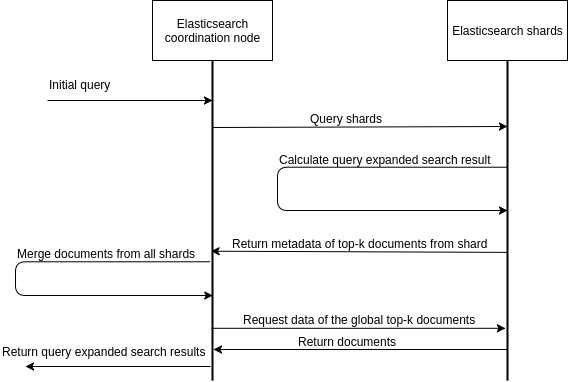
\includegraphics[width=0.9\linewidth]{img/sequence-diagram-elasticsearch.png}
\caption{Sequence diagram for the Elasticsearch implementation.}
\label{fig:sequence-diagram-lucene}
\end{figure}

\section{Query Expansion Implementation}
Algorithm explanation.

\section{Web Server}
